\documentclass{../../text-style}

\texttitle{Лекция 6: Управление проектами, часть 1}

\begin{document}

\maketitle
\thispagestyle{empty}

\attribution{Тимофей Александрович Брыксин, бывш. доцент кафедры системного программирования СПбГУ}

\section{Управление проектами}

Прежде чем начинать говорить об управлении проектами, нужно объяснить, что же такое проект. Классическое управление проектами выделяет два вида организации человеческой деятельности: операционная и проектная.

Операционная деятельность применяется, когда внешние условия хорошо известны и стабильны, когда производственные операции хорошо изучены и неоднократно испытаны, а функции исполнителей определены и постоянны. В этом случае основой эффективности служат узкая специализация и повышение компетенции.

Там, где разрабатывается новый продукт, внешние условия и требования к которому постоянно меняются, где применяемые производственные технологии используются впервые, где постоянно требуются поиск новых возможностей, интеллектуальные усилия и творчество, там требуются проекты.

Таким образом, проект --- это временное предприятие, предназначенное для создания уникальных продуктов, услуг или результатов. В отличие от операционной деятельности, процесс которой можно строго формализовать и лишь следить за грамотным его исполнением, проектной деятельности требуется постоянное внимание. Управление проектом --- это сложная и ресурсозатратная деятельность, которая жизненно важна для успеха проекта. Её рассмотрением мы и займёмся.

\section{Критерии успеха проекта}

В любой деятельности необходимо понимать критерии её успешности и критерии неудачи. В проектной деятельности можно выделить пять основных критериев успеха:

\begin{itemize}
    \item Соглашение между ключевыми участниками о целях проекта. Данный критерий совершенно очевиден, тем не менее существует множество проектов, развитие которых происходит без понимания конечной цели проекта. В любом проекте всегда пытайтесь добиться, чтобы все ключевые участники были согласны с целями проекта. Заметим, что причиной неудачи проекта может оказаться разное понимание терминов, составляющих цель проекта. Убедитесь не только в том, что все ключевые участники согласны с целями, но и в том, что понимание целей проекта у всех участников единообразное. И это понимание сохраняется по ходу развития проекта.
    \item План как средство отслеживания прогресса проекта. План позволит вам не только распределить обязанности по задачам в проекте (и в нужный момент найти места, которые стоит усилить), но и отслеживать общий прогресс проекта. Достаточно детализированный план послужит ранним сигналом об отставании задач от графика и позволит предпринять меры по устранению риска.
    \item Эффективные коммуникации. Помните, что люди выполняют проекты, а не планы. Обеспечьте максимальную эффективность коммуникаций, как формальных, так и неформальных. Помните, что любой вклад в коммуникации между людьми --- одна из самых разумных инвестиций для вас, как для руководителя проекта.
    \item Управляемые границы проекта. С самого начала проекта и до его завершения все вовлечённые в проект участники должны понимать границы того, что может быть реализовано при текущих временных рамках и текущем бюджете. Особенно важно понимать границы проекта, если его ход подразумевает внесение изменений в требования и постановку задачи.
    \item Правильные люди на правильных местах. Вы должны понимать границы компетенций ваших сотрудников и грамотно распоряжаться людскими ресурсами. Не заставляйте дизайнера разрабатывать frontend, и не заставляйте frontend-разработчика рисовать логотип, даже если их компетенции близки. Ну только если совсем другого выбора нет или по согласованию и при заинтересованности самих работников.
\end{itemize}

Важно понимать, что все перечисленные критерии должны применяться не только к непосредственным исполнителям проекта --- разработчикам, но и к лицам, заинтересованным в проекте (заказчики, менеджемент). Если главная угроза со стороны разработчиков для вас --- некачественная реализация требуемой функциональности (или её отсутствие), то главная угроза со стороны менеджмента --- изменение условий проекта (бюджета, временных рамок, требований). Если не поддерживать связи с ними, не описывать им границы проекта, то однажды бюджет проекта могут урезать вдвое, и тут вас не спасет ни одна прекрасно коммуницирующая команда.

Вообще, всё что мы перечислили ранее так или иначе связано с различными областями ответственности менеджера. Рассмотрим их подробнее.

\section{Функции менеджера проекта}

По сути своей функции менеджера проекта разделяются на три больших группы --- определение задач проекта, планирование проекта и контроль проекта. Рассмотрим их более подробно.

\begin{center}
    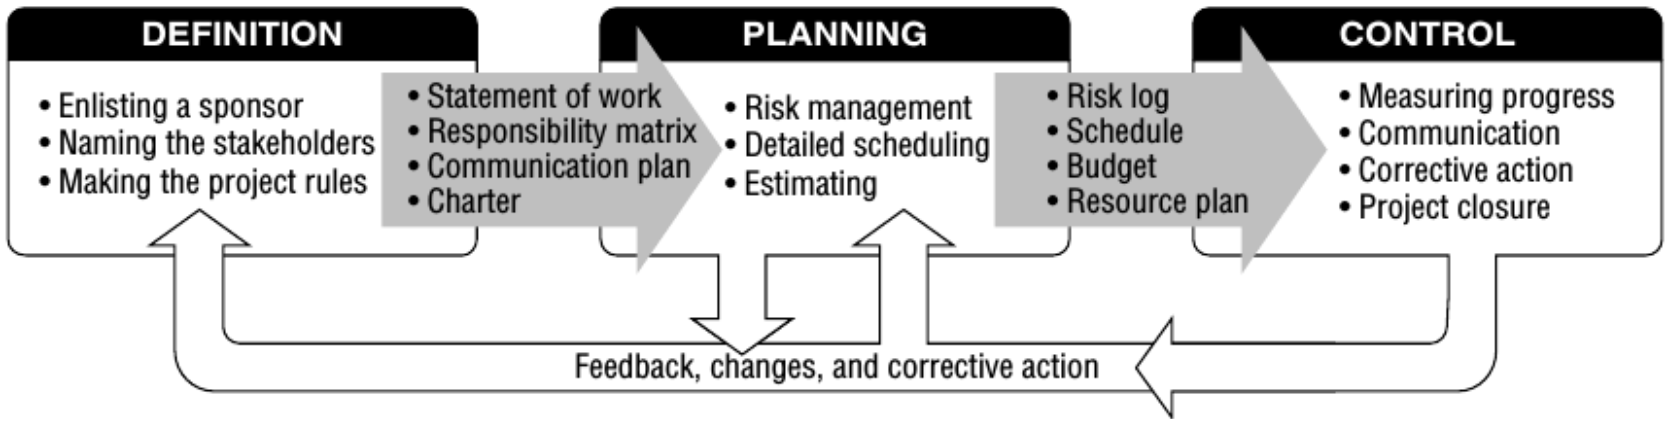
\includegraphics[width=0.9\textwidth]{projectManagerFunctions.png}
\end{center}

При старте проекта менеджер должен определить задачи проекта (возможно, при помощи аналитиков) и достичь по ним соглашения с заказчиками и менеджментом. Также на этой стадии менеджер должен определить основных вовлеченных в разработку субъектов, их роли и ответственности. Все созданные на данной стадии документы становятся своего рода <<правилами игры>>: они определяют, как играть и что нужно, чтобы выиграть.

На стадии планирования проекта составляется детальный план проекта, оцениваются объемы вовлеченных ресурсов, планируется график проекта с учётом имеющихся ограничений. Также на этой стадии производится планирование рисков.

На стадии контроля проекта менеджер должен поддерживать проект на пути к цели. На этой стадии менеджер измеряет прогресс проекта, устраняет возникающие риски и корректирует, при необходимости, план проекта.

Все эти стадии выполняются друг за другом: сначала определяется суть проекта, потом производится планирование, затем проект запускается и осуществляется контроль за его ходом. Но при этом постоянно происходит и возврат к предыдущим стадиям: детальное планирование ведёт к лучшему пониманию сути проекта, а действия по управлению часто требуют пересмотра плана (а то и всего проекта в целом).

Теперь более подробно рассмотрим участников проекта.

\section{Stakeholders (заинтересованные субъекты)}

В каждом проекте есть так называемые стейкхолдеры --- это люди, заинтересованные в проекте по той или иной причине. К ним относятся не только заказчики и пользователи (заинтересованность которых совершенно понятна), но и сам менеджер проекта, высший менеджмент и команда разработки. Все они являются ключевыми участниками проекта и согласие между всеми ними --- обязательный критерий успешности проекта. По сути главная задача менеджера проекта --- удовлетворение потребностей всех заинтересованных лиц. Но при этом каждый из них должен и вносить что-то своё в развитие проекта, и задача менеджера проекта создать для этого все условия. Если какая-то (любая) из групп стейкхолдеров перестанет выполнять свои функции, проекту будет крайне сложно завершиться успешно.

Разберем роли, ответственности каждой из этих групп.

\subsection{Менеджер проекта}

Задача менеджера проекта --- определить роли всех заинтересованных субъектов, определить задачи проекта и определить критерии удовлетворения потребностей остальных стейкхолдеров, включая себя самого. Всё это обсуждалось ранее. 

\subsection{Команда проекта}

Команда проекта --- это люди, которые выполняют основную часть работы. Тем не менее у каждого человека в команде роли разные. Кто-то быстро нарисует логотип проекта и уйдёт в следующий, а кто-то будет с проектом от начала до конца.

Первой задачей менеджера станет набрать команду, определить основные компетенции, которые потребуются, и сколько нужно специалистов каждого типа, на какой срок. Также в его обязанности входит построить механизмы коммуникации с командой и внутри неё.

Кроме того, менеджер должен обеспечить команде доступ к работникам с другими компетенциями, чтобы выполнять изредка возникающую работу. Такие работники не будут в ядре команды, однако их придется приглашать, и обеспечить возможность для этого --- задача менеджера.

\subsection{Менеджмент}

Менеджмент --- это люди, которые способны своим решением существенно повлиять на проект. При планировании проекта менеджеру проекта нужно учитывать как возможности, так и угрозы со стороны менеджмента. В частности, нужно понимать, кто и чем может помочь, а кто имеет право на закрытие проекта, на урезание бюджета и т.д. Все эти вопросы кажутся неважными лишь до тех пор, пока менеджер проекта, проект или кто-то из команды не начнёт испытывать какие-то сложности. Вот тут и пригодится вся накопленная информация.

\subsection{Спонсор/покровитель}

В большинстве случаев в компании имеется более высокопоставленный, чем менеджер проекта, человек, заинтересованный в успешном развитии проекта. Это может быть один из директоров, инвестор или кто-то ещё. Часто по ходу проекта у менеджера может просто не хватать возможностей для того, чтобы принять некоторые жизненно важные для проекта решения (например, выделение дополнительного бюджета, использование каких-то особых ресурсов или людей с уникальными компетенциями и т.п.). В этом случае подобный спонсор может быть крайне полезен, помогая обходить острые углы в иерархии управления организации или помогая своим опытом менеджеру в управлении проектом. 
Менеджеру важно понять, если ли у его проекта такой покровитель, и если есть, то какова его заинтересованность, и чем он может помочь. Человек, который высказывает заинтересованность, но никак не включается в проект, не особо полезен.

\subsection{Заказчик}

Определить заказчика иногда далеко не так тривиально, как могло бы показаться. К примеру, в задачи вашего проекта входит установка какого-нибудь специального софта на все компьютеры в организации. Кто заказчик этого? Менеджмент? Все 360 работников? В таком случае менеджер проекта должен пойти дальше и задать вопрос не <<Кто заказчик?>>, а <<Кто определяет требования и оплачивает результат?>>. В таких случаях стейкхолдерами оказываются и заказчик, и конечные потребители продукта.

Все эти роли важно понимать и предусматривать риски, связанные с ними. Иначе можно оказаться в ситуации, когда к завершению проекта вы уже год как не разговариваете с менеджером из соседнего отдела, потому что поругались из-за парковочного места, а он ответственен за допуск вашего проекта к выпуску.

Повторим ещё раз: каждый человек из заинтересованных в проекте лиц имеет свои потребности и должен что-то привносить в проект. Задача менеджера на начальном этапе проекта --- определить и зафиксировать этот круг людей, а затем строить взаимодействия с ними по ходу проекта для достижения лучших результатов. Важно также понимать, кто не входит в список заинтересованных лиц, и чьё мнение о проекте не так важно, чтобы всё бросать и начинать делать что-то другое в соответствии с ним.

\section{Матрица ответственностей}

Как правило, кроме формального или неформального описания стейкхолдеров, относящихся к той или иной роли, менеджеру полезно также построить так называемую матрицу ответственностей.

\begin{center}
    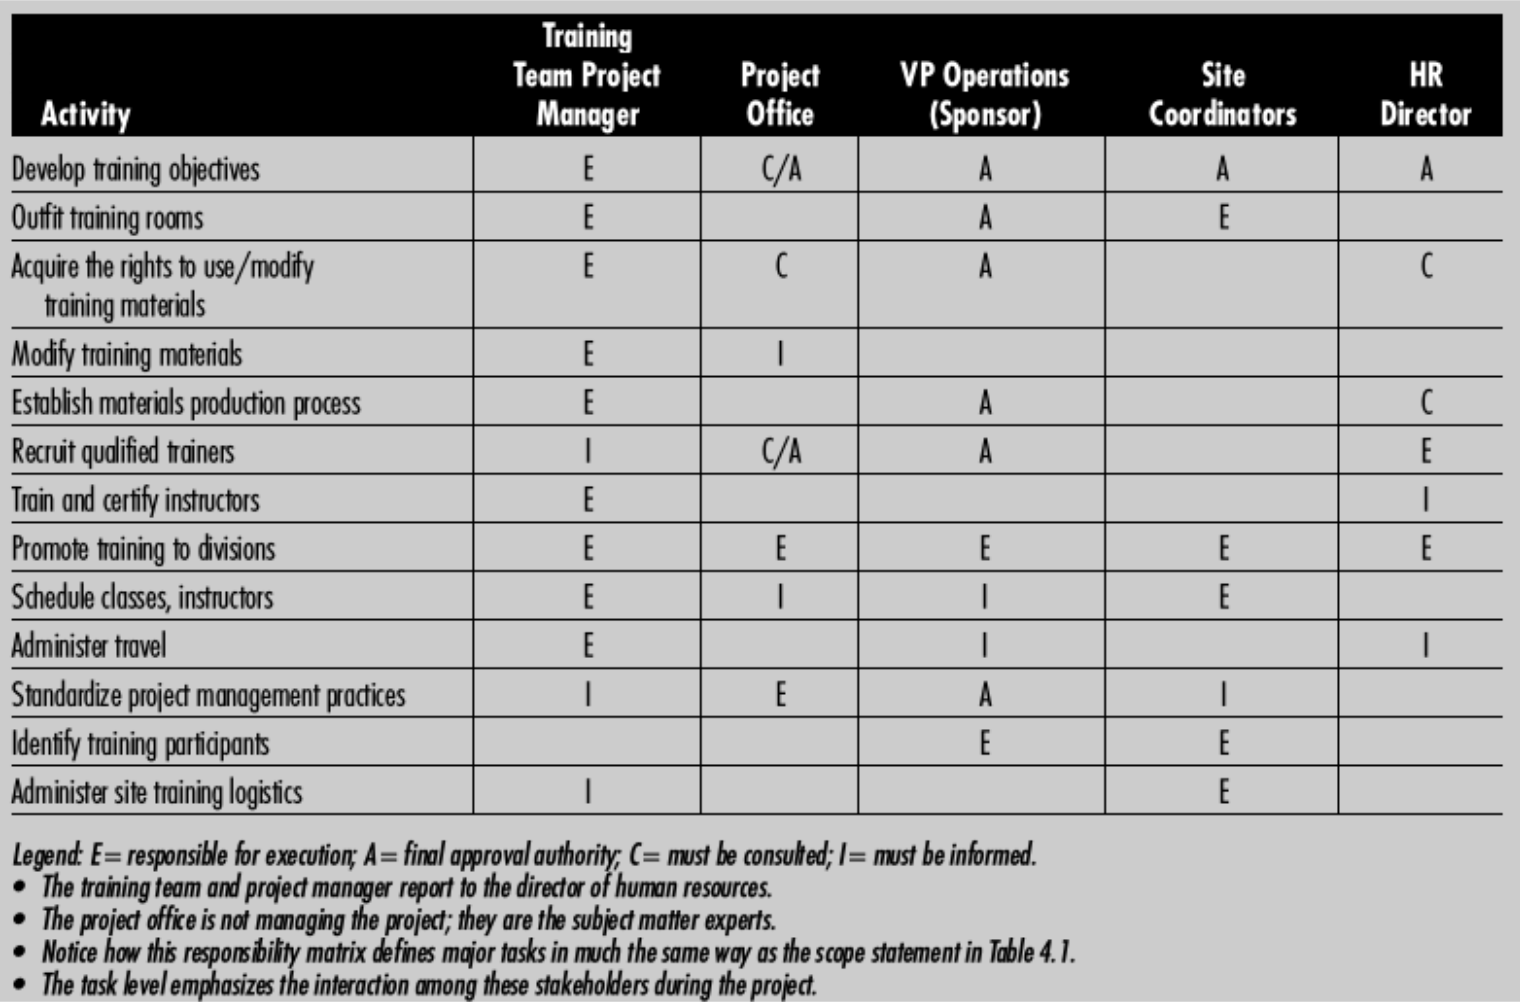
\includegraphics[width=0.9\textwidth]{stakeholders.png}
\end{center}

Эта матрица по горизонтали содержит стейкхолдеров, а по вертикали основные виды деятельности, предпринимаемые в проекте. На пересечении вы можете указать, что нужно предпринять по отношению к данному человеку или группе людей при решении той или иной задачи: уведомить, проконсультироваться, получить разрешение и т.д. Такая матрица --- довольно мощный инструмент, позволяющая в любой момент понимать, по каким каналам должны осуществляться коммуникации в проекте, и кто за что в рамках каких задач отвечает.

К тому же, с помощью данной матрицы можно производить согласования с конкретными стейкхолдерами об объеме их вовлечения в проект. По крайней мере, не лишним будет показать эту матрицу всем заинтересованным лицам и получить их согласие и одобрение относительно ваших планов на них. Заручившись согласием с этим планом всех ключевых лиц, можно избежать большого числа недоразумений и разногласий.

Создавать такой документ нужно как можно раньше, пока ещё проект не начался. Потом, когда у каждого из ключевых лиц сформируется своё мнение о происходящих процессах, вам будет гораздо сложнее что-то исправить.

\section{Коммуникационный план}

Кроме матрицы ответственностей полезно составить так называемый коммуникационный план. В нём указываются, каким стейкхолдерам нужна какая информация в какие периоды времени. Рассмотрим его и вообще процессы коммуникаций более подробно.

\begin{center}
    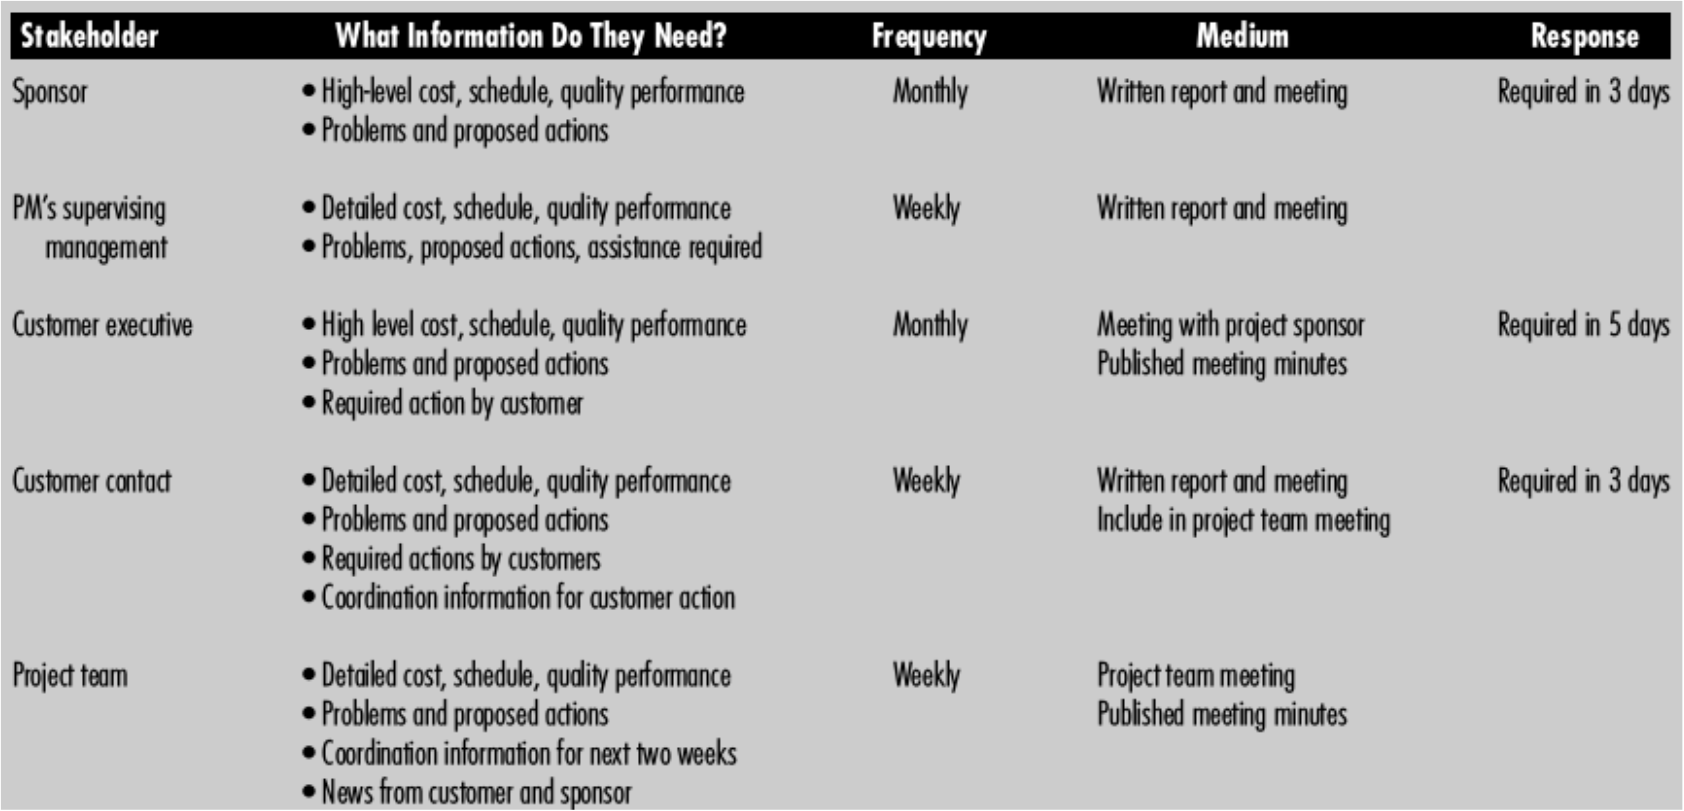
\includegraphics[width=0.9\textwidth]{communicationPlan.png}
\end{center}

\subsection{Status report}

Составление отчета о статусе проекта куда сложнее, чем может показаться на первый взгляд.

Во-первых, необходимо определиться с тем, какую информацию о статусе проекта требуется отправлять каждому стейкхолдеру. Очевидно, директорату не особо интересно, что программист Вася заболел, и его обязанности должен исполнить Петя, но это крайне важно для Пети. При составлении коммуникационного плана в специальной графе напротив каждого стейкхолдера указывается, какая информация должна доводиться до его сведения.

Во-вторых, необходимо определиться с регулярность отчетов. Нет необходимости заваливать стейкхолдеров горами информации, они просто перестанут её читать.

Вы должны отправлять отчёт ровно так часто, чтобы каждый из стейкхолдеров получал необходимую ему информацию к необходимому ему времени. Тут во многом сказывается опыт менеджера, потому как очень легко посчитать какие-то детали незначительными и не включить их в отчёт, а если бы начальство таки получило эту информацию, они могли бы предотвратить какую-нибудь проблему. Найти эту грань довольно сложно, для директората это может быть отчет раз в неделю, а для участников команды --- митинг каждый день, однако найти её необходимо. Во многом от этого будет зависеть эффективность коммуникации в вашей команде.

В-третьих, вы должны определиться с формой отчета для каждого из стейкхолдеров. Некоторых из них удовлетворятся письмом, другие же должны посещать митинги. Очень соблазнительно перевести всё в онлайн, однако надо помнить, что даже если человек подключен к вашему скайп-звонку, это совсем не значит, что он сидит и всё внимательно слушает. Впрочем, про личное присутствие на совещании можно сказать похожие вещи.

Наконец, зафиксируйте время ожидания ответов на отчеты о статусе, если ответы ожидаются.

В итоге, правильно составленный коммуникационный план позволит вам всегда быть в курсе текущих коммуникаций в проекте и быть уверенным, что все стейкхолдеры обладают всей необходимой информацией и отслеживают развитие проекта.

\subsection{Дополнительные запросы}

К запросам, не относящимся к отчётам о статусе проекта (таким как запрос на разрешение какого-либо вида деятельности, на увеличение ресурсов и т.д.) применяются ровно те же правила, что и к отчётам о статусе. Правильно выбирайте человека, пишите по теме и правильно выбирайте время. Но с этим обычно проще, поскольку запрос и есть запрос, важно только не забыть указать контекст, в котором вы его делаете. 

\subsection{Эскалация}

Отдельно отметим необходимость формализации процесса эскалации --- передачи ответственности на более высокий уровень иерархии (антипод делегирования). Заранее составленный (в идеале согласованный) план эскалации даёт гарантию того, что в критический момент вы будете знать, к кому обратиться из менеджмента, и что он/она для вас сможет сделать.

\section{Планирование}

Мы рассмотрели основные активности, предпринимаемые до стадии планирования. К этому моменту вы уже выделили роли стейкхолдеров, создали план коммуникаций и набросали матрицу ответственностей. Теперь рассмотрим задачи, выполняемые непосредственно на стадии планирования. Она состоит из двух больших видов деятельности, которые между собой очень сильно переплетены: это анализ рисков и планирование. 

\subsection{Управление рисками}

Риски --- это любые неприятные события, которые могут случиться по ходу проекта. Как правило, они разделяются на <<известное неизвестное>> и <<неизвестное неизвестное>>. Под <<известным неизвестным>> понимаются события, суть которых нам известна, однако неизвестно, произойдут они или нет. Такими рисками можно управлять, о чём мы поговорим далее. Под <<неизвестным неизвестным>> понимаются события, суть которых неизвестна, как и неизвестно, произойдут они или нет. С такими рисками бороться нельзя, как правило на них закладывают дополнительные ресурсы и надеются, что их хватит.

Само понятие управления рисками --- это систематическая работа по выявлению рисков, их классификации и их устранению. Чрезвычайно важно здесь то, что эта работа систематическая: чем систематичнее ваш подход к рискам, тем лучше вы можете их контролировать. И когда что-то плохое случится, у вас уже будет заготовлен план противодействия.

Можно даже сказать, что управление рисками --- основная работа менеджера. Причём на стадии планирования детальное планирование проекта и управления рисками идут рука об руку. Вы начинаете планировать новую задачу, выявляете риски этой задачи, определяете стратегию их устранения (о чём далее) и ставите задачу в план. То есть каждая задача при планировании должны быть оценена не только с точки зрения ресурсов, графика и т.д., но и с точки зрения возможных рисков.

Теперь пошагово разберем процесс управления рисками:

\begin{center}
    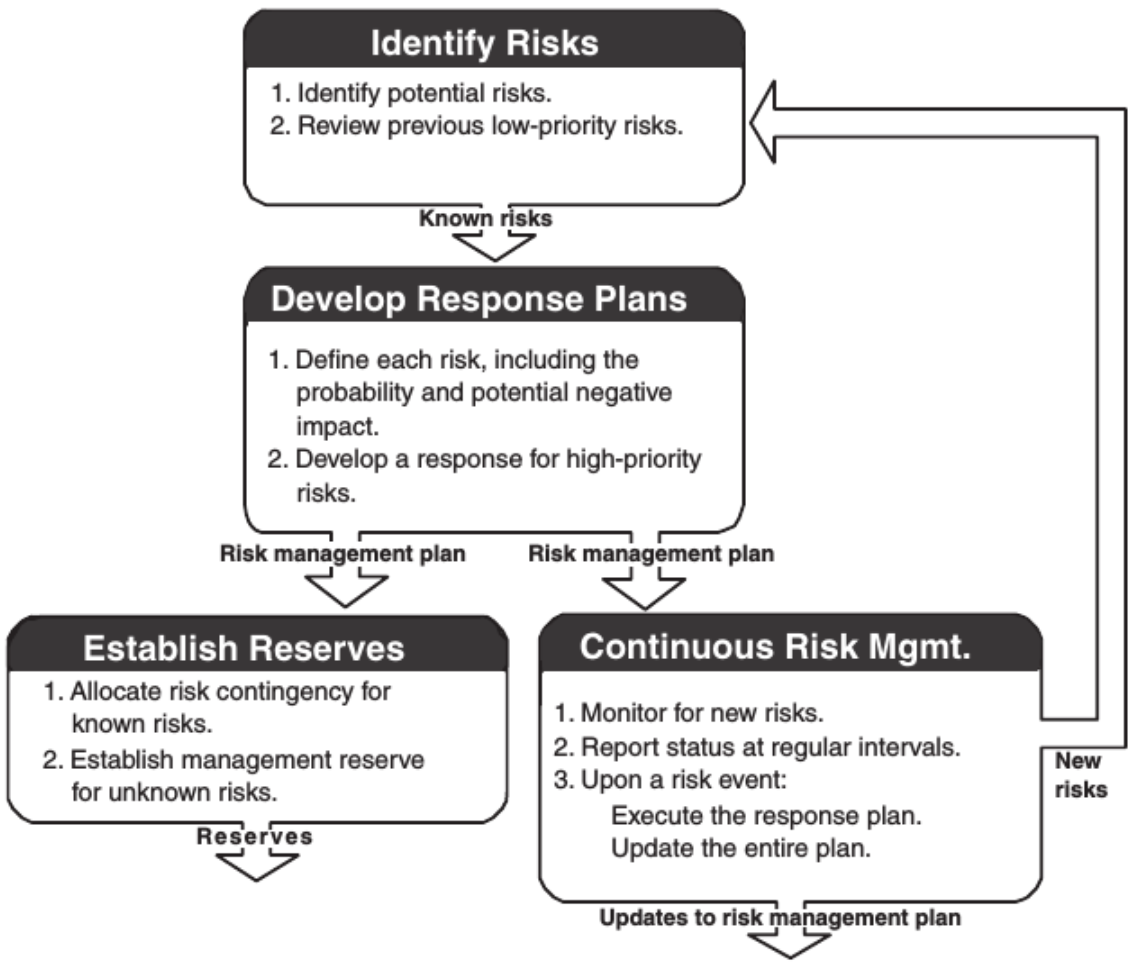
\includegraphics[width=0.7\textwidth]{riskManagementLoop.png}
\end{center}

\subsubsection{Распознавание риска}

На первой стадии управления рисками их необходимо идентифицировать. Для этого можно использовать разные методы, начиная от опроса стейкхолдеров и заканчивая привлечением статистических данных.

При опросе стейкхолдеров менеджер собирает их мнения относительно предполагаемых рисков, после чего анализирует полученную информацию. Менеджер выявляет возможные риски, группирует их по степени важности и вероятности и удаляет повторения. Данный анализ можно также проводить не через интервьюирование, а через мозговые штурмы. Тут важно записывать вообще всё, что только приходит в голову: потом риски можно будет приоритизировать и отбросить совсем уж маловероятные.

Другой подход --- использовать профиль риска. В случае, если в компании производились похожие проекты, по ним должны были быть составлены специальные опросники, выявляющие наиболее часто встречающиеся в проектах такого типа риски --- профили рисков. Используя их, вы можете выявить часть рисков. По окончании проекта предполагается, что вы также обновите профили риска новой информацией, полученной из данного проекта.

Можно использовать прошлый опыт и напрямую. Поднимите в архивах документацию по прошлым проектам такого типа. Графики, составленные их менеджерами, и реальные графики исполнения проектов дадут ценную информацию относительного того, что может пойти не так.

Наконец, часть рисков вы обнаружите прямо в ходе планирования. Просто отмечайте те задачи, которые трудно спланировать по времени и/или бюджету. Почти наверняка они содержат тот или иной фактор риска.

После того, как вы выявили риск, опишите его. Укажите условия при которых он может произойти и последствия, которые он повлечет. Удостоверьтесь, что из вашего описания ясно, в чём состоит риск, каковы его последствия, можно ли его избежать, и, если можно, то каких ресурсов это потребует. Помните, что чем детальнее вы определите риски и возможные последствия, тем лучше вы сможете риском управлять. Поэтому, данной части стоит уделить особое внимание.

К примеру, описание <<В проекте нам придётся работать с технологией, с которой ни у кого из разработчиков нет опыта работы>> довольно плохое. Понятно, что это риск, но как с ним бороться, по описанию даже предположить сложно. Его можно было записать иначе: <<Заказчик требует интеграцию нашего приложения с его информационными системами по протоколу X, с которым в команде никто ранее не работал>>. Такое описание более чётко описывает проблему и даёт возможность рассматривать варианты её решения.

Постарайтесь назначить риску некоторую вероятность. Определить её можно, исходя из статистических данных или из опыта. К сожалению, трудно формализовать процесс вычисления вероятности риска. В случае, если невозможно произвести более или менее строгую количественную оценку, можно произвести субъективную качественную оценку. Это менее точный вариант, однако это лучше, чем не оценивать вероятность риска вовсе. Привлекайте к оценке экспертов в этой области, человек без понимания ситуации даст гораздо менее надёжную оценку.

\subsubsection{Выработка стратегия противодействия}

При разработке стратегии противодействия нужно учитывать как вероятности риска, так и тяжесть его последствий. Если последствия и вероятность оценены количественно, то можно перемножить их и получить некоторую абсолютную величину опасности риска. В случае, если оценки производились качественно, можно использовать квадрат рисков.

\begin{center}
    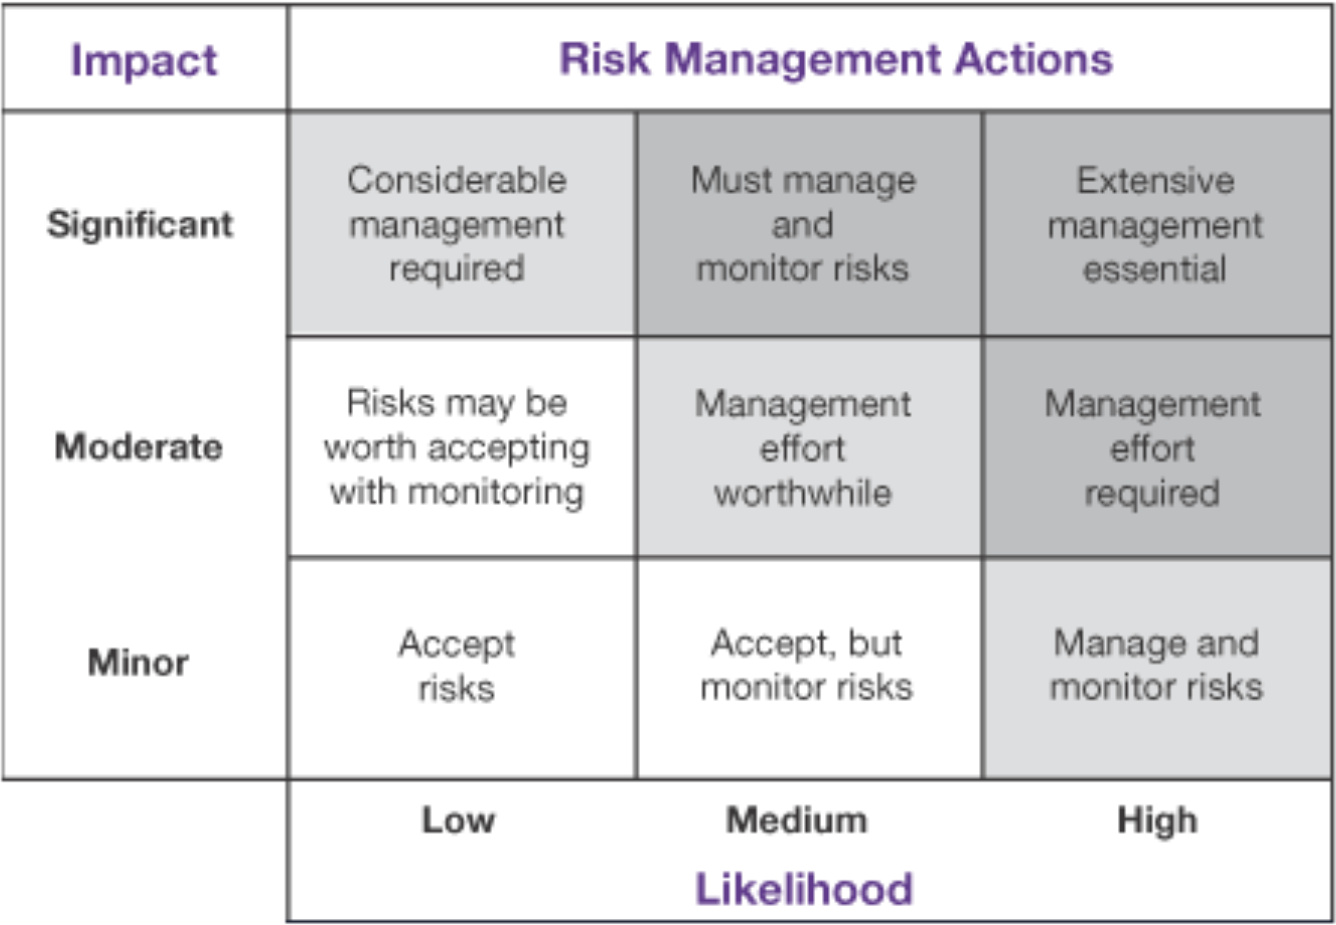
\includegraphics[width=0.6\textwidth]{riskMatrix.png}
\end{center}

Чем ближе риск к правому верхнему углу, тем риск <<опаснее>>, чем ближе к левому нижнем, тем он более <<безопасен>>.

Классифицировав некоторым образом риск по его опасности, можно применить к нему одну из стратегий противодействия рискам.

\emph{Принять риск.} Вы понимаете риск, его последствия, и решаете его принять, то есть не производить никаких активных действий по его устранению. Такая стратегия, как правило, применяется либо если риск находится в нижнем левом угле квадрата, либо если затраты на противодействие ему больше затрат на устранение последствий (и при этом они вписываются в бюджет).

\emph{Избежать риска.} Вы понимаете риск и решаете отказаться от реализации части системы, порождающей его. Как правило, такая стратегия применяется, если риск вероятен, его последствия велики, а предотвратить его стоит излишне дорого. Но тут нужно быть осторожным, поскольку велика вероятность лишить свой продукт одного из конкурентных преимуществ. Как правило, чем больше риск реализации чего-то, тем больше пользы это что-то приносит.

\emph{Переложить риск.} Вы понимаете риск и решаете предоставить возможность разобраться с ним приглашенному специалисту или вообще отдать эту задачу на аутсорсинг. Нужно понимать, что при этом риск и его последствия не исчезают, но контролировать его вы больше не можете. Это уже не ваша ответственность, но всё ещё ваша головная боль. К тому же, вы получаете новые риски взаимодействия с экспертами/субподрядчиками.

\emph{Смягчить риск.} Вы понимаете риск и решаете провести сейчас некоторые дополнительные работы, смягчающие его возможные последствия (к примеру, если есть риск, что команда не успеет разобраться в новой технологии, то вы можете пригласить эксперта по ней, чтобы он провел мастер-класс).

\emph{Отслеживать риск.} Вы понимаете риск и решаете отслеживать вероятность его возникновения. В случае, если вероятность возникновения риска достигнет какого-то критического значения, вы начнете предпринимать активные действия по его предотвращению. Однако, при отслеживании риска важно понимать, насколько мы в состоянии адекватно отслеживать и предсказывать его появление. Если риск из вероятного превратится в наступивший в течении пары секунд, вариант с отслеживанием не для вас. Но и если риск будет медленно наступать в течение пары лет, у вас должен быть чёткий критерий того, что риск уже случился, и нужно начинать ему противодействовать. Ситуация будет напоминать историю про лягушку, сварившуюся в кастрюле\footnote{\url{https://ru.wikipedia.org/wiki/Лягушка_в_кипятке}}.

Результаты анализа рисков и построения стратегий противодействия имеет смысл организовать в таблицу. Например, такого формата:

\begin{center}
    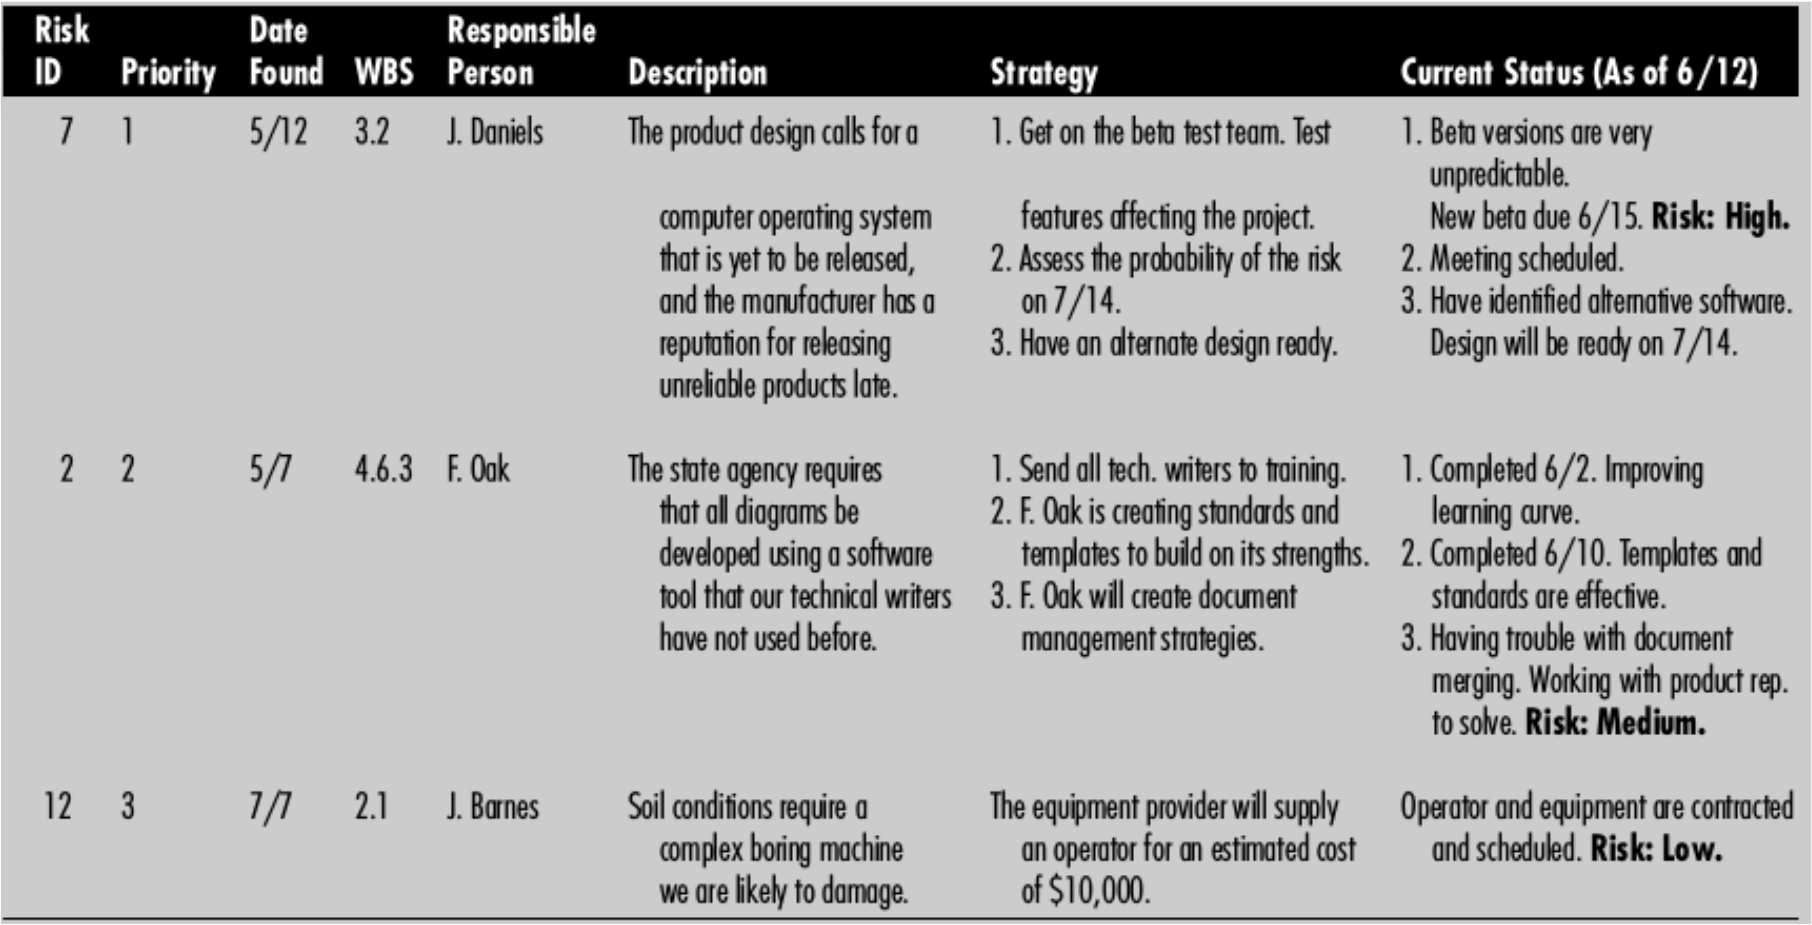
\includegraphics[width=\textwidth]{riskExample.png}
\end{center}

Здесь указываются не только риски и их приоритетность, но и ответственные и статус самого риска.

\subsubsection{Создание резервного фонда}

Противодействие рискам требует бюджета. Очень маловероятно, что получится сформировать такой резервный фонд, которые будет покрывать все описанные риски вообще (крайне маловероятно, что сразу случится вообще всё плохое, что только может), поэтому чаще всего компромисс достигается путём анализа, предположений и переговоров. Как правило, вычисляют размер этого фонда следующим образом: отбирается наиболее вероятная часть рисков, вероятность этих рисков умножается на стоимость противодействия им и складывается, к результирующей сумма прибавляется 5-50\% от бюджета проекта на неизвестные риски. Процент на неизвестные риски зависит от специфики проекта, опыта компании, команды и лично менеджера. 

\subsubsection{Непрерывное управление рисками}

Но на этом всё не заканчивается. После старта проекта менеджер должен постоянно отслеживать риски, оценивать их и предлагать стратегии противодействия. Соответственно, задачей менеджера становится:

\begin{itemize}
    \item отслеживать текущие риски;
    \item выявлять новые риски, оценивать их и предлагать стратегии противодействия;
    \item проводить регулярную полную переоценку рисков на предопределенных стадиях проекта (например, завершение прототипа, выход нового релиза и т.д.). Собственно, эту информацию удобно отображать в колонке <<статус>> в предыдущей таблице.
\end{itemize}

Непрерывное управления рисками гарантирует, что менеджер всегда будет в курсе текущих рисков проекта и сможет грамотно на них отреагировать.

\subsection{Декомпозиция проекта}

Другой стадией планирования является декомпозиция проекта. Невозможно анализировать сложный проект, рассматривая его как целое --- как правило требуется сначала разбить его на части/подзадачи и лишь потом анализировать.

Достаточно маленькую подзадачу уже можно проанализировать и спланировать: определить затраты ресурсов, риски исполнения и роли стейкхолдеров, которые должны будут принять участие в реализации задачи. С помощью декомпозиции можно получить достаточно точный и детализированный план выполнения проекта.

Представлять разбиение задач можно в графической или текстовой форме. Графическая более наглядна, но может быть неудобна в использовании при большом количестве задач. 

\begin{center}
    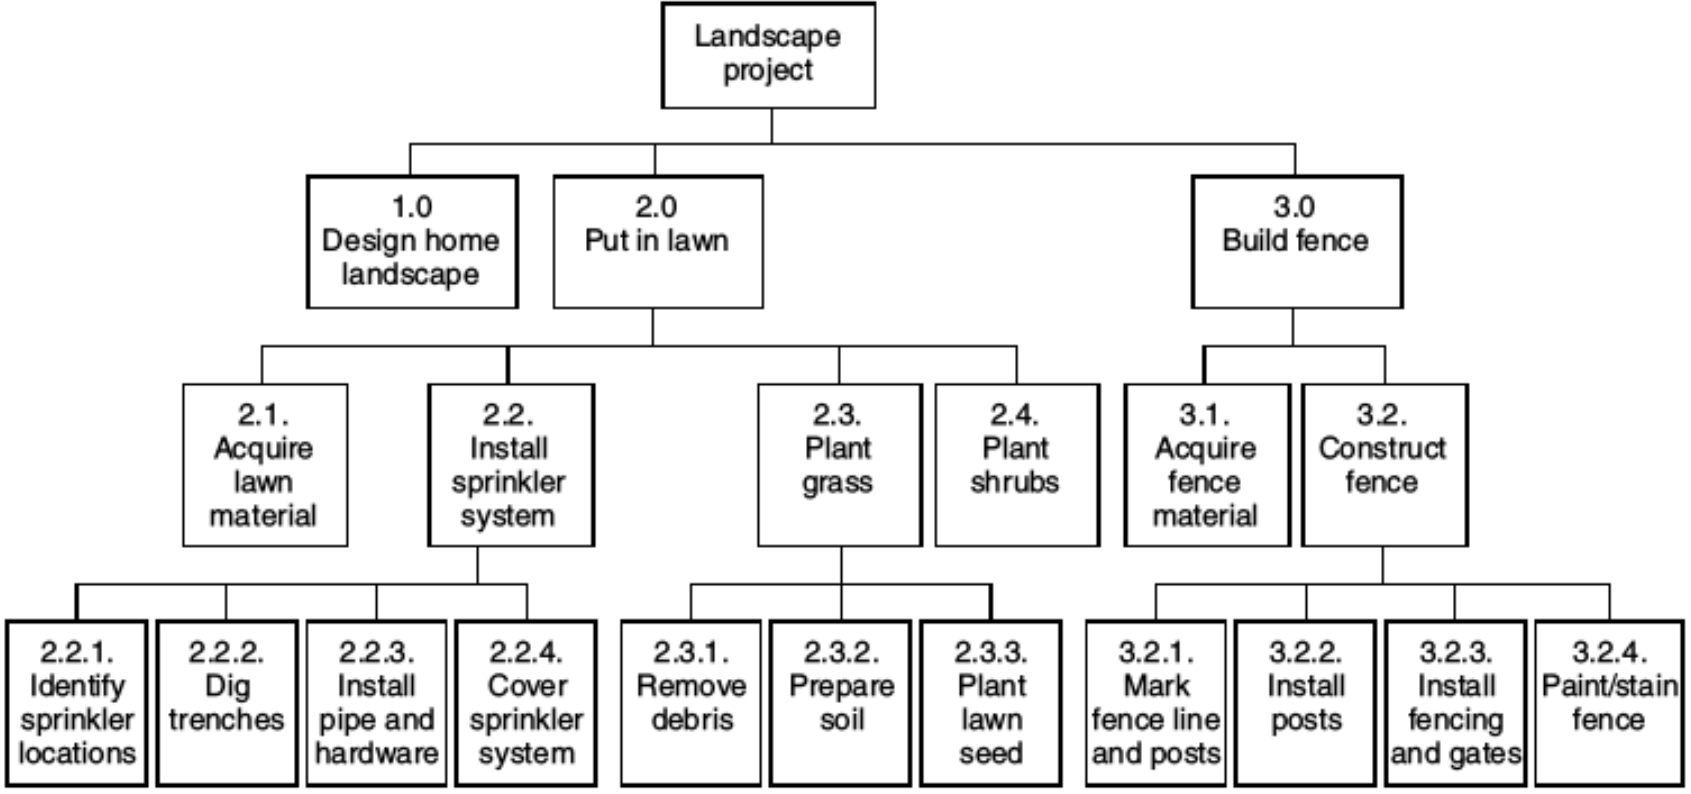
\includegraphics[width=\textwidth]{wbsExample.png}
\end{center}

\begin{center}
    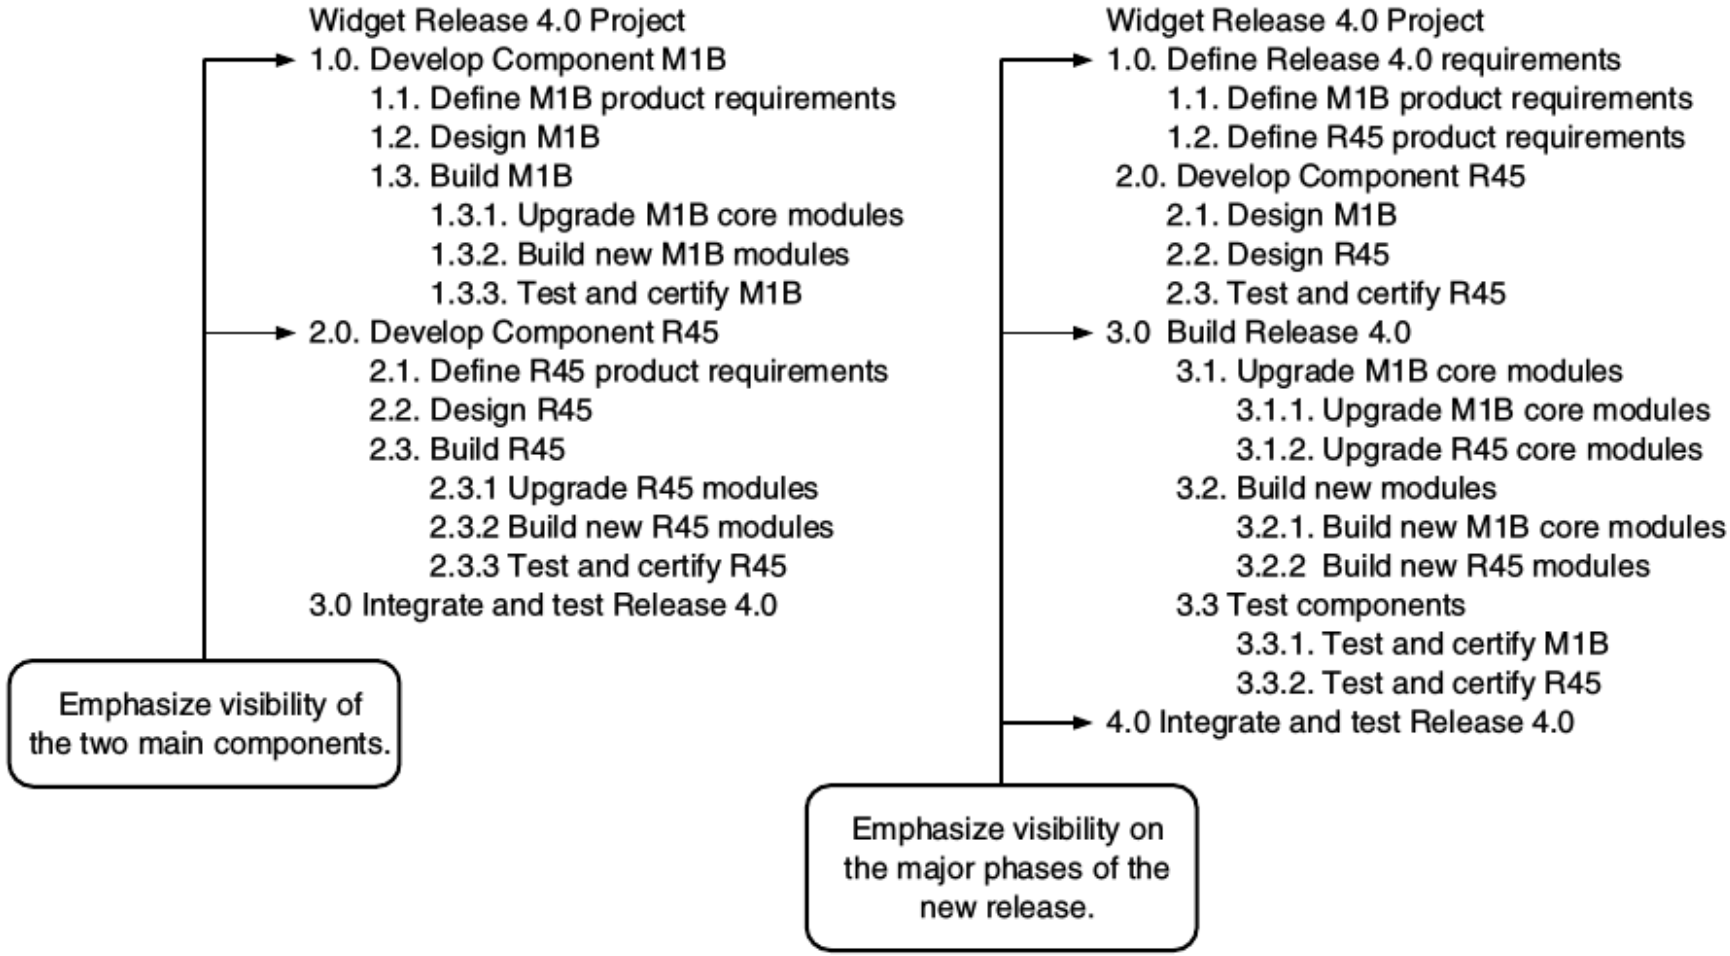
\includegraphics[width=0.9\textwidth]{wbsExample2.png}
\end{center}

Качественное дерево задач можно использовать для иллюстрации границ проекта и для отслеживания прогресса. В дальнейшем дерево декомпозиции будет основой для построения плана проекта и оценки его длительности и необходимого бюджета.

\subsubsection{Методы декомпозиции}

Декомпозицию можно делать по-разному. Во-первых, это может быть нисходящая декомпозиция: вы берёте абстрактную задачу (например, сделать такой-то продукт) и разбиваете её до тех пор, пока не получите вполне конкретные задачи по производству конкретных частей данного продукта. Эти задачи должны быть настолько малы, что вы легко можете их анализировать, оценивать и понимаете процесс исполнения этих задач (если вы не понимаете процесс, который стоит за этой задачей, то привлеките экспертов). Итоговые задачи можно переупорядочить и получить общий процесс выполнения проекта. Другой подход --- идти от высокоуровневых видов деятельности, которые нужно совершить (см. левый и правый вариант списка на рисунке выше), и дальше разбивать их на более мелкие работы.

Во-вторых, восходящая: вы рассматриваете конкретные задачи по созданию частей продукта и уже из них собираете сам продукт.

Заметим, что не всякая декомпозиция должна быть полной. Каждой команде или стейкхолдеру проекта на самом деле требуется некоторая проекция на декомпозицию --- её модель, скрывающая все ненужные детали и подчеркивающая важные. Важно это понимать и не слать на каждый запрос плана проекта полную схему, а предоставлять лишь то, что действительно нужно.

\subsubsection{Критерии хорошей декомпозиции}

Если декомпозиция нисходящая, то каждая подзадача должна действительно быть подмножеством объемлющей задачи. В случае, если это не так, то декомпозиция просто неверна. Также все дети задачи в сумме должны давать саму задачу. Это тоже обязательное условие корректности декомпозиции.

Описание задачи должно явно содержать глагол, который определяет ключевую деятельность и явное существительное, которая определяет главный артефакт. <<Протестировать модуль A>>, <<Реализовать модуль B>>, <<Спроектировать модуль C>>. То есть такие задачи, которые потом можно будет поместить в таск-трекер и раздавать членам команды. Примеры плохих задач: <<Провести исследование>>, <<База данных>>.

\subsubsection{Размеры конечных задач}

Определение размеров конечных задач --- вопрос чрезвычайно субъективный. Размеры задач зависят от вашего опыта в планировании, размеров проекта и ресурсов, выделенных для планирования проекта. Тем не менее, есть некоторые общие рекомендации.

Есть известное <<правило 8/80>>: согласно ему, работа над задачей должна занимать не менее восьми и более восьмидесяти часов.

В случае, если в вашей организации есть некоторые установленные периоды отчетности (например, еженедельные доклады о статусе проекта), то удобно, чтобы задачи занимали не более, чем два отчёта. В таких случаях вы не окажетесь в ситуации, когда на докладе о статусе разработчик будет говорить, что сделано 37\%. Задача будет либо сделана, либо нет.

Также при выборе размеров конечных задач стоит руководствоваться здравым смыслом. При размере задач в 15 человеко-минут спланировать проект будет стоить чрезвычайно дорого, а сам процесс будет очень неэффективен из-за постоянного микроменеджмента. Та же проблема и со слишком большими задачами.

К тому же, при изменении целей или деталей проекта некоторые участки дерева задач могут оказаться больше неактуальными. Так что при декомпозиции стоит соблюдать разумный баланс в объёме задач в листьях дерева.

\subsubsection{Задачи по управлению проектом}

Не забывайте включать в дерево задач само управление проектом. Это тоже работа, и она должна быть учтена при распределении времени и ресурсов. Есть единичные задачи (например, провести семинар, заказать футболки), их более-менее логично явно обозначить в дереве, а повторяющиеся задачи (например, постоянная переоценка рисков, рассылка отчётов стейкхолдерам и т.п.) имеет смысл собрать в одну общую задачу <<Управление проектом>>.

\end{document}
